\section{Stability and Bifurcation analysis}
Analysis of system can be divided in two section:
\begin{itemize}
    \item $R_0 < 1$
    \item $R_0 > 1$
\end{itemize}

\begin{theorem}
\label{th:sir_equilibria}
The vector field \ref{eq:sir_model_3} has a not endemic equilibrium point $x_{ne}^* = (1,0)$ and an endemic equilibrium point $x_e^*=(\frac{1}{R_0}, \frac{\mu}{\beta} (R_0 - 1))$.
\end{theorem}

\begin{proof}
To get equilibria of \ref{eq:sir_model_3} it is mandatory verify that vector field is null \cite[p. 3]{bib:khalil}.

\begin{equation}
\label{eq:sir_model_nullclines_1}
         \mu - \beta x_sx_i - \mu x_s = 0
\end{equation}

\begin{equation}
\label{eq:sir_model_nullclines_2}
         \beta x_sx_i - (\gamma + \mu)x_i = 0
\end{equation}

From \ref{eq:sir_model_nullclines_2} we get

\begin{equation}
\label{eq:sir_model_nullclines_2_demonstation}
         \beta x_sx_i - (\gamma + \mu)x_i = (\beta x_s -\gamma - \mu)x_i
\end{equation}

THat is equal to 0 for $x_i = 0$ e $x_s = \frac{\gamma + \mu}{\beta}=\frac{1}{R_0}$

If $x_i = 0$ from \ref{eq:sir_model_nullclines_1} we get $x_s = 1$, that corresponds to not endemic equilibrium point $x_{ne}^*$.

If $x_s = \frac{1}{R_0}$ from \ref{eq:sir_model_nullclines_1} we get $x_i=\frac{\mu}{\gamma + \mu} - \frac{\mu}{\beta} = \frac{\mu}{\beta} (R_0 - 1)$, that corrisponds to endemic equilibrium point $x_e^*$.
\end{proof}

First of all, willbe usefull calculate Jacobian matrix of system \ref{eq:sir_model_3}.

\begin{equation}
    J = 
    \begin{pmatrix}
        \frac{\partial \dot{x_s}}{\partial x_s} & \frac{\partial \dot{x_s}}{\partial x_i} \\
        \frac{\partial \dot{x_i}}{\partial x_s} & \frac{\partial \dot{x_i}}{\partial x_i}
    \end{pmatrix} =
    \begin{pmatrix}
        -\mu-\beta x_i & \beta x_s \\ \beta x_i & \beta x_s -(\gamma + \mu)
    \end{pmatrix}
\end{equation}

Eigenvalues of generic point $(x_s,x_i)$ are

\begin{equation}
    \label{eq:eigenvalues}
    \lambda = 
    \begin{vmatrix}
        \lambda + \mu + \beta x_i & \beta x_s \\
        -\beta x_i & \lambda - \beta x_s  (\gamma + \mu)
    \end{vmatrix}
    = (\lambda + \mu + \beta x_i)(\lambda - \beta x_s + \gamma + \mu ) + \beta^2 x_s x_i
\end{equation}

In not endemic equilibrium point eigenvalues are

\begin{equation}
    \label{eq:eigenvalues_ne}
    (\lambda + \mu)(\lambda - \beta + \gamma + \mu) = 0 \implies \lambda_1 = - \mu, \lambda_2 = \beta-\gamma-\mu
\end{equation}

While, in endemic equilibrium point eigenvalues are

\begin{equation}
    \label{eq:eigenvalues_e}
    \lambda^2+\lambda\left(\frac{\beta\mu}{\gamma + \mu}\right)+\mu(\beta-\gamma-\mu) = 0 \implies \lambda_{1,2} = -\frac{\beta\mu}{2(\gamma + \mu)} \pm \frac{1}{2}\sqrt{\left(\frac{\beta\mu}{\gamma + \mu}\right)^2-4\mu(\beta-\gamma-\mu)}
\end{equation}

First of continue, will be usefull calculates divergence of system \ref{eq:sir_model_3}.

\begin{equation}
\label{eq:divergence}
    \nabla\bullet f = \frac{\partial f_1}{dx_s} + \frac{\partial f_2}{dx_i}=-\mu+\beta (x_s - x_i) -(\gamma + \mu)=\beta\left[(x_s - x_i) - \left(\frac{\mu}{\beta} + \frac{1}{R_0}\right)\right]
\end{equation}

\subsection{Analysis for $R_0 < 1$}
\subsubsection{Existence of equilibria}
\begin{theorem}
\label{th:R0_minor_then_1_Equilibria}
Suppose that $R_0 < 1$, then System (\ref{eq:sir_model_3}) has one hyperbolic equilibrium point (not endemic equilibrium) that is locally asymptotically stable (node).
\end{theorem}

\begin{proof}
For endemic equilibrium point happens that

\begin{equation}
    x_s^* = \frac{1}{R_0}
\end{equation}

By assumption

\begin{equation}
    R_0 < 1 \implies x_s^* > 1 \implies x_e^* \not\in \Omega
\end{equation}

For not endemic equilibrium point is obvious verify that $x_{ne}^* \in \Omega$.

Given Equation (\ref{eq:eigenvalues_ne}) and, remembering that by assumption $\mu > 0$ and $\gamma > 0$

\begin{equation}
    \lambda_1 = -\mu < 0
\end{equation}

\begin{equation}
    \lambda_2 = \beta - \gamma - \mu = (\gamma + \mu)\left(\frac{\beta}{\gamma + \mu} - 1\right) = (\gamma + \mu)(R_0 - 1) < 0
\end{equation}

So not endemic equilibrium point has real negative eigenvelus, so is a node.
\end{proof}
\subsubsection{Existence of limit cycle}
\begin{theorem}
Suppose that $R_0 < 1$. So in $\Omega$ don't exist isolated periodic solution.
\end{theorem}

\begin{proof}
Is obvious verify that $\Omega$ is a simply connected domain.

Moreover, from equation \ref{eq:divergence} is possible verify that divergence of vector field \ref{eq:sir_model_3} is equal to zero in 

\begin{equation}
    (x_s - x_i) - \left(\frac{\mu}{\beta} + \frac{1}{R_0}\right) = 0 \implies (x_s - x_i) = \left(\frac{\mu}{\beta} + \frac{1}{R_0}\right) 
\end{equation}

But, by assumption

\begin{equation}
    R_0 < 1 \implies (x_s - x_i) = \left(\frac{\mu}{\beta} + \frac{1}{R_0}\right) > 1 \implies x_s > x_i + 1 \geq 1
\end{equation}

For each point $\left(x_s,x_i\right) \in \Omega$ happens that 

\begin{equation}
    x_s \leq 1
\end{equation}

So equation \ref{eq:divergence} cannot be equal to zero (and, consequently change sign) in a simply connected domain. For Bendixson-Dulac criterion \cite[pp.~67]{bib:khalil} don't exist isolated periodic solution in $\Omega$ .
\end{proof}

\begin{figure}[h!]
    \centering
    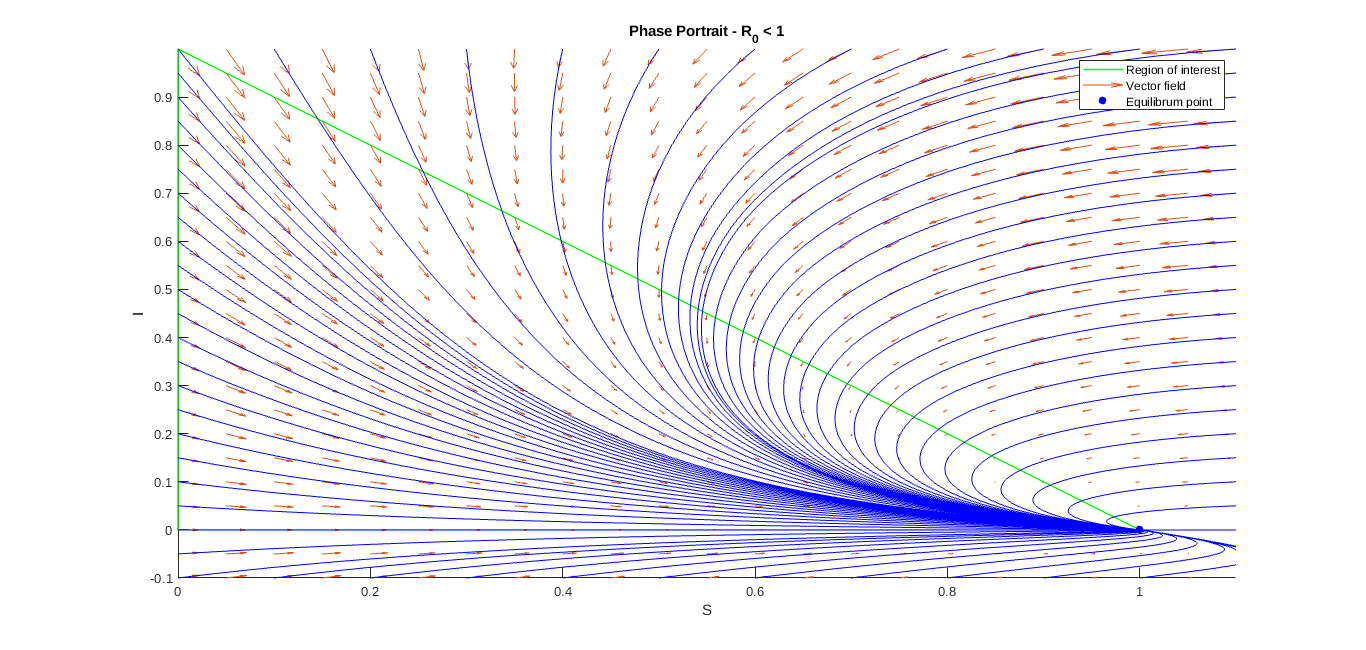
\includegraphics[scale=0.45]{Figure/pp_R0_minor_1.png}
    \caption{Phase Plane of SIR model with $R_0 < 1$ and parameters $\beta = 0.4$, $\mu = 0.2$, $\gamma=0.3$}
    \label{fig:phase_plane_r0_minor_1}
\end{figure}

\subsubsection{Stability analysis}
\begin{theorem}
Suppose that $R_0 < 1$. So not endemic equilibrium point is asymptotically stable in $\Omega$.
\end{theorem}

\begin{proof}
Choosing as candidate Lyapunov function

\begin{equation}
    \label{eq:lyapunov_r0_minor_1}
    V = x_i + P \;\;\;\;\; P > 0
\end{equation}

it happens that

\begin{equation}
    \label{eq:lyapunov_derivative_1_r0_minor_1}
    \dot{V} = \frac{\partial V}{\partial x_s} \dot{x_s} + \frac{\partial V}{\partial x_i} \dot{x_i} = \beta x_sx_i-\left(\gamma+\mu\right)x_i=x_i\left(\gamma+\mu\right)\left(R_0x_s-1\right)
\end{equation}

Now

\begin{itemize}
    \item $V > 0 \;\;\;\;\; \forall \left( x_s, x_i \right) \in \Omega$
    \item $ \dot{V} \leq 0 \;\;\;\;\; \forall \left( x_s, x_i \right) \in \Omega$
    \item $ \dot{V} = 0 \implies M = \{(x_s,x_i) \in \mathbb{R}^2: x_i = 0\}$
    \item Largest invariant set in $M$ is $E = \{(x_s^*,x_i^*)\}$
\end{itemize}

Moreover, for $x_i = 0$ it happnes that
\begin{equation}
    \dot{x_s} = \mu - \mu xs \implies x_s=-c(x_s(0))e^{-\mu t}+1
\end{equation}
and
\begin{equation}
    t \rightarrow +\infty \implies x_s \rightarrow 1
\end{equation}

So for Corollary of Krasowskii of LaSalle invariant principle, not endemic equilibrium point is asymptotically stable in $\Omega$. \cite[p.128]{bib:khalil}
\end{proof}
\begin{figure}[h!]
    \centering
    \label{fig:lyapunov_r0_minor_1}
    \begin{subfigure}{\textwidth}
        \centering
        % include first image
        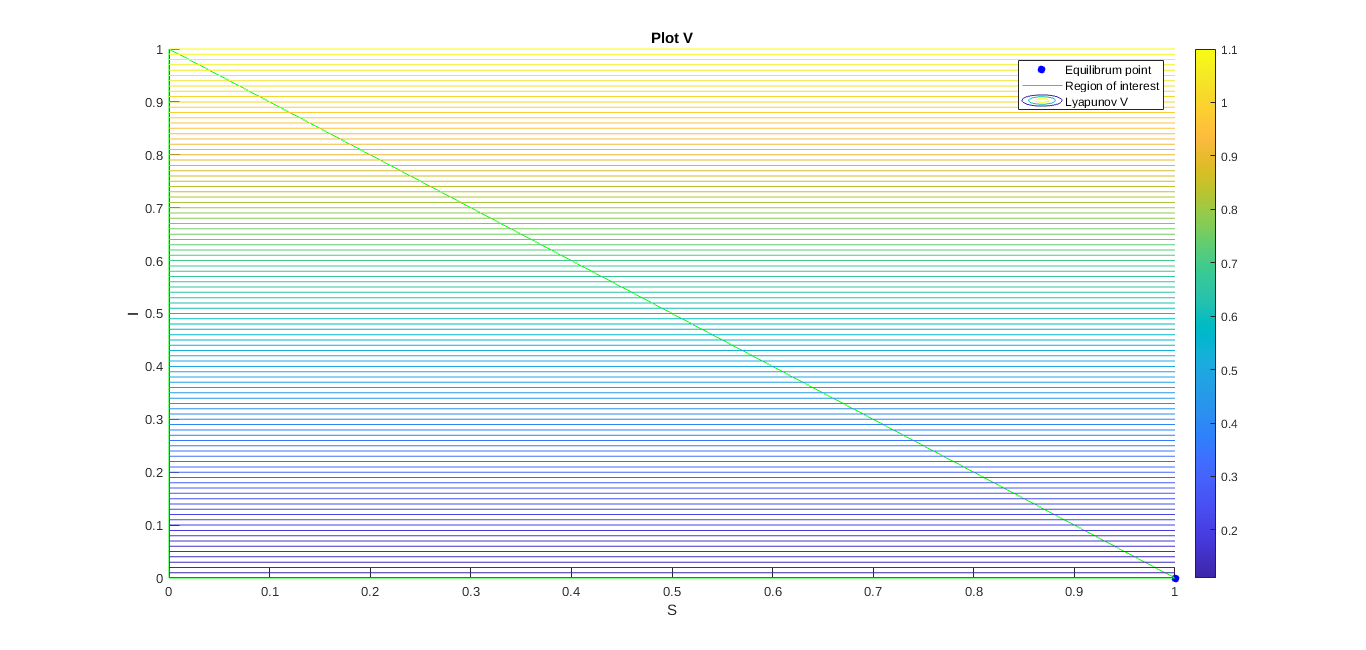
\includegraphics[width=\linewidth]{Figure/lyapunov_2d_R0_minor_1.png}  
        \caption{V in 2D}
        \label{fig:lyapunov_r0_minor_1_first}
    \end{subfigure}
    \begin{subfigure}{\textwidth}
        \centering
        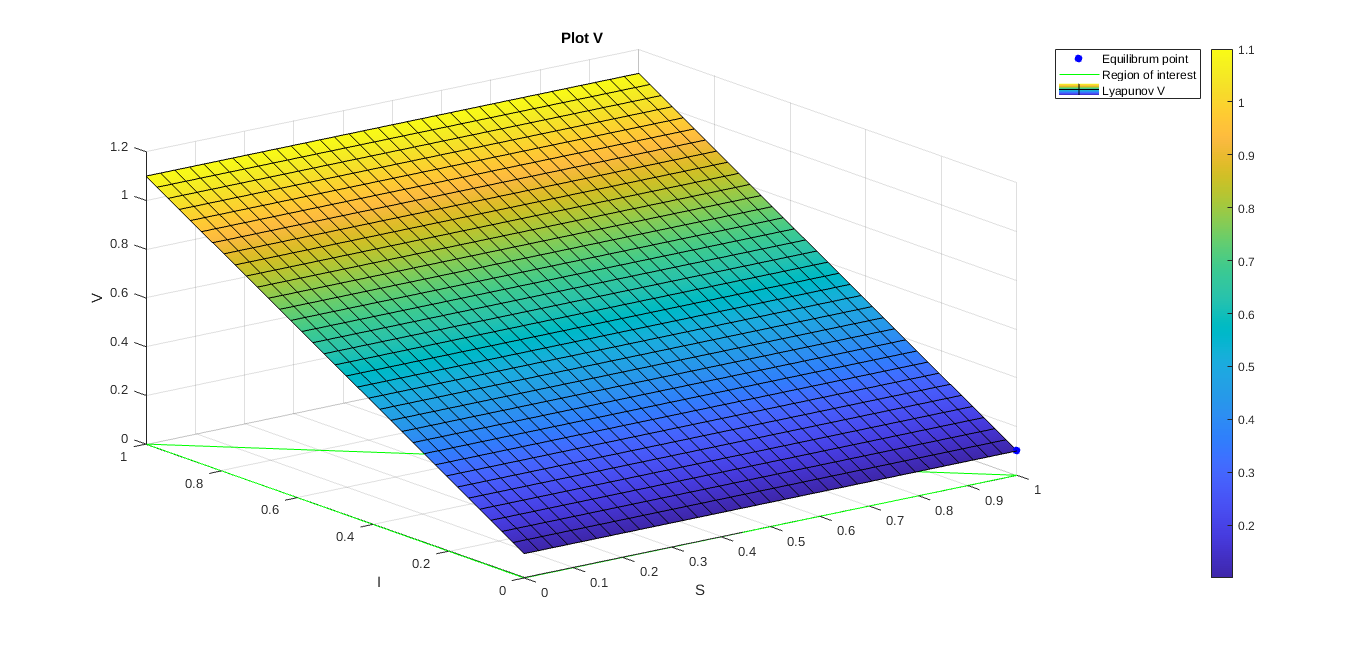
\includegraphics[width=\linewidth]{Figure/lyapunov_3d_R0_minor_1.png}  
        \caption{V in 3D}
        \label{fig:lyapunov_r0_minor_1_second}
    \end{subfigure}
    \caption{V with parameters $\beta = 0.4$, $\mu = 0.2$, $\gamma = 0.3$, $P = 0.1$}
\end{figure}

\begin{figure}[h!]
    \centering
    \label{fig:lyapunov_derivative_r0_minor_1}
    \begin{subfigure}{\textwidth}
        \centering
        % include first image
        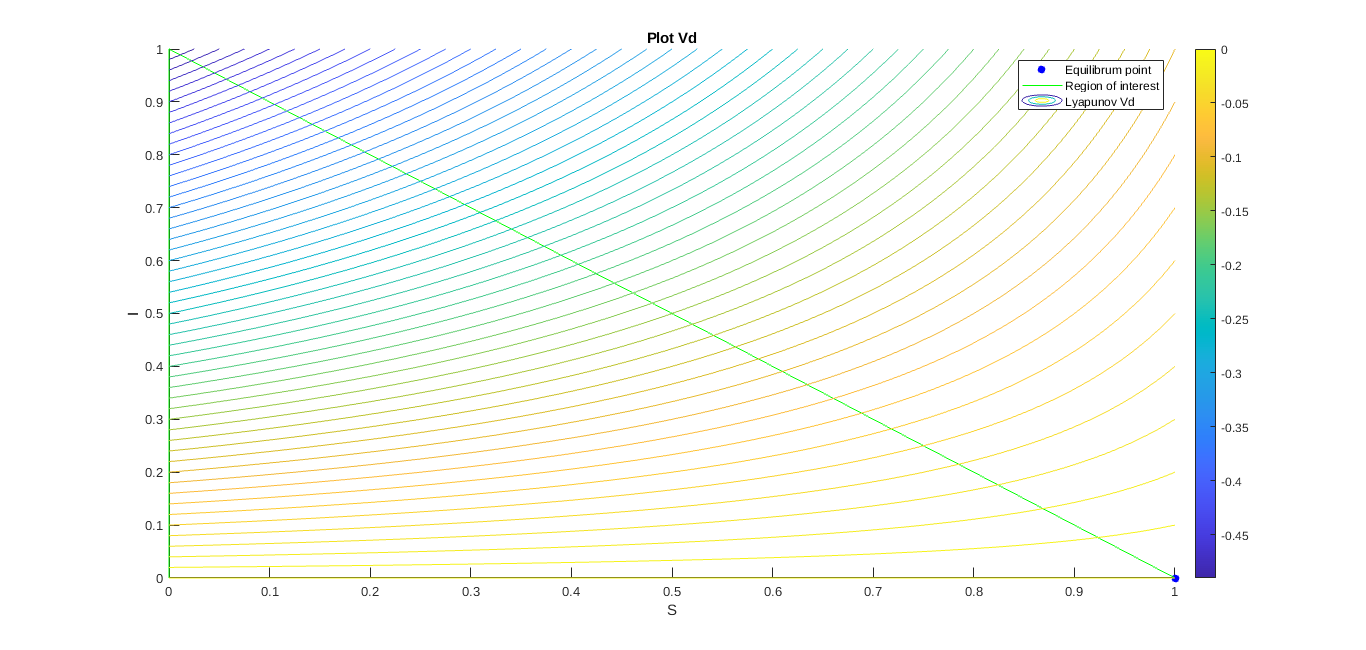
\includegraphics[width=\linewidth]{Figure/lyapunov_derivative_2d_R0_minor_1.png}  
        \caption{$\dot{V}$ in 2D}
        \label{fig:lyapunov_derivative_r0_minor_1_first}
    \end{subfigure}
    \begin{subfigure}{\textwidth}
        \centering
        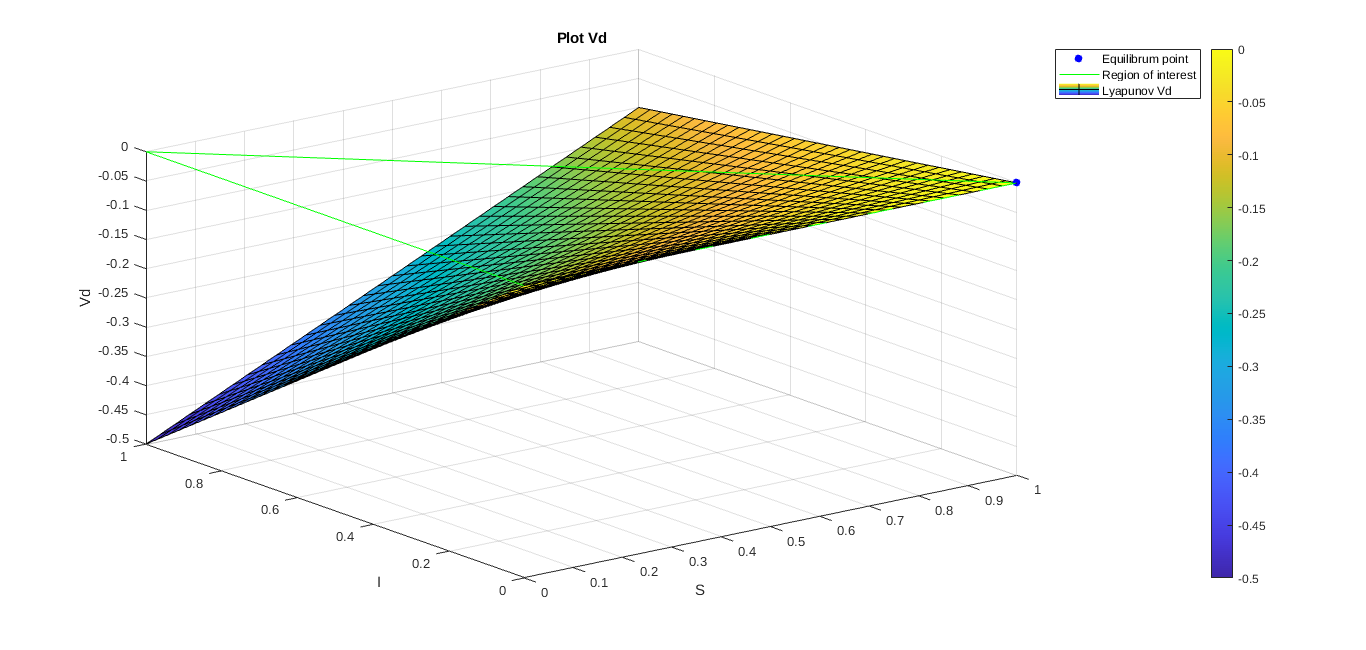
\includegraphics[width=\linewidth]{Figure/lyapunov_derivative_3d_R0_minor_1.png}  
        \caption{$\dot{V}$ in 3D}
        \label{fig:lyapunov_derivative_r0_minor_1_second}
    \end{subfigure}
    \caption{$\dot{V}$ with parameters $\beta = 0.4$, $\mu = 0.2$, $\gamma = 0.3$, $P = 0.1$}
\end{figure}

\break
\subsection{Analysis for $R_0 > 1$}
\subsubsection{Existence of equilibria}
\begin{theorem}
\label{th:R0_major_then_1_Equilibria}
Given $R_0 > 1$, then System (\ref{eq:sir_model_3}) has two equilibrium point that are not endemic equilibrium point (saddle point) and endemic equilibrium point (locally asymtotically stable).
\end{theorem}

\begin{proof}
Considering not endemic equilibrium point. It obvious verify that $x_{ne}^* \in \Omega$.

Given Equation (\ref{eq:eigenvalues_ne}) and remembering that by assumption $\mu > 0$ and $\gamma > 0$, so

\begin{equation}
    \lambda_1 = -\mu < 0
\end{equation}

\begin{equation}
    \lambda_2 = \beta - \gamma - \mu = (\gamma + \mu)\left(\frac{\beta}{\gamma + \mu} - 1\right) = (\gamma + \mu)(R_0 - 1) > 0
\end{equation}

Then not endemic equilibrium point has a real positive eigenvalue and a real negative eigenvalue, so is a saddle point.

Now considering the endemic equilibrium point. First of all it is mandatory verify that this point is a part of domain $\Omega$.

\begin{equation}
    x_s^* = \frac{1}{R_0}
\end{equation}

But, by assumption

\begin{equation}
    R_0 > 1 \implies x_s^* < 1
\end{equation}

Moreover, 

\begin{equation}
    x_s^* < 0 \implies R_0 < 0  
\end{equation}

But this cannot be true because $R_0 > 1$ by assumption. In the end

\begin{equation}
    x_s^* = 0 \implies 0 = 1  
\end{equation}

and this is a contraddiction. So

\begin{equation}
    0 < x_s^* < 1
\end{equation}

For $x_i^*$

\begin{equation}
    1 < R_0 = \frac{\beta}{\gamma + \mu} \implies \frac{1}{\beta} < \frac{1}{\gamma + \mu} \implies 0 < \frac{1}{\gamma + \mu} - \frac{1}{\beta} \implies 0 < \frac{\mu}{\gamma + \mu} - \frac{\mu}{\beta} = x_i^*
\end{equation}

Moreover

\begin{equation}
    1 < R_0 = \frac{\beta}{\gamma + \mu} \implies \beta > \gamma + \mu > \mu \implies x_i^* = \frac{\mu}{\gamma + \mu} - \frac{\mu}{\beta} < 1 - \frac{\mu}{\beta} < 1
\end{equation}

In the end

\begin{equation}
    x_s^* + x_i^* = \frac{1}{R_0} + \frac{\mu}{\beta}\left(R_0 - 1\right) < \frac{1}{R_0} + \frac{\mu+\gamma}{\beta}\left(R_0 - 1\right) =  \frac{1}{R_0} + \frac{1}{R_0}\left(R_0 - 1\right) = 1
\end{equation}

So

\begin{equation}
    0 < x_s^* < 1, \;\; 0 < x_i^* < 1, \;\; x_s^* + x_i^* < 1 \implies x_e^* \in \Omega 
\end{equation}

Now it need to analyze eigenvalues. Substituiting Equation (\ref{eq:r0_definition}) in Equation (\ref{eq:eigenvalues_e}) it happens:

\begin{equation}
    \lambda_{1,2} = -\frac{\mu R_0}{2} \pm \frac{1}{2}\sqrt{\left(\mu R_0\right)^2-\frac{4\mu}{\gamma + \mu}(R_0 - 1)}
\end{equation}

Now, it happnes that

\begin{equation}
    \left(\mu R_0\right)^2-\frac{4\mu}{\gamma + \mu}(R_0 - 1) = \left(\mu R_0\right)^2-\frac{4\mu R_0}{\beta}(R_0 - 1)
\end{equation}

Noting that

\begin{equation}
    R_0 > 1 \implies -\frac{4\mu R_0}{\beta}(R_0 - 1) < 0
\end{equation}

So it can happen only three possible scenarios:

\begin{itemize}
    \item $1 < R_0 < \frac{4}{4-\beta \mu} \implies \lambda_{1,2}$ are complex conjugate eigenvalues with negative real part (stable focus)
    
    \item $R_0 = \frac{4}{4-\beta \mu} \implies \lambda_{1,2}$ are coincident negative real eigenvalues (attractive star)
    
    \item $R_0 > \frac{4}{4-\beta \mu} \implies \lambda_{1,2}$ are distinct negative real part ( node )
\end{itemize}

In all three scenarios eingevalues have negative real part, so equilibrium point is an hyperbolic equilibrium point locally asymptotically stable.
\end{proof}
\subsubsection{Existence of limit cycle}
For $R_0 > 1$ is not possible use the Bendixson - Dulac criterion because in $\Omega$ there is an equilibrium point that is locally asymptotically stable, ed removing this point from domain, $\Omega$ became a not simply connected domain.

It could apply Poincaré - Bendixson Theorem to search periodic solution, but in section dedicated to stability analysis will be show that for $R_0 > 1$ endemic equilibrium point is locally asymptotically stable in $\Omega_c \subset \Omega$, where $\Omega_c = \{\left(x_s,x_i\right) \in \mathbb{R}^2 : x_s > 0, x_i > 0, x_s + x_i < 1\}$, so there cannot be periodic solution in $\Omega$. This result is showed in Figure \ref{fig:phase_plane_r0_major_1}.

\begin{figure}[h!]
    \centering
    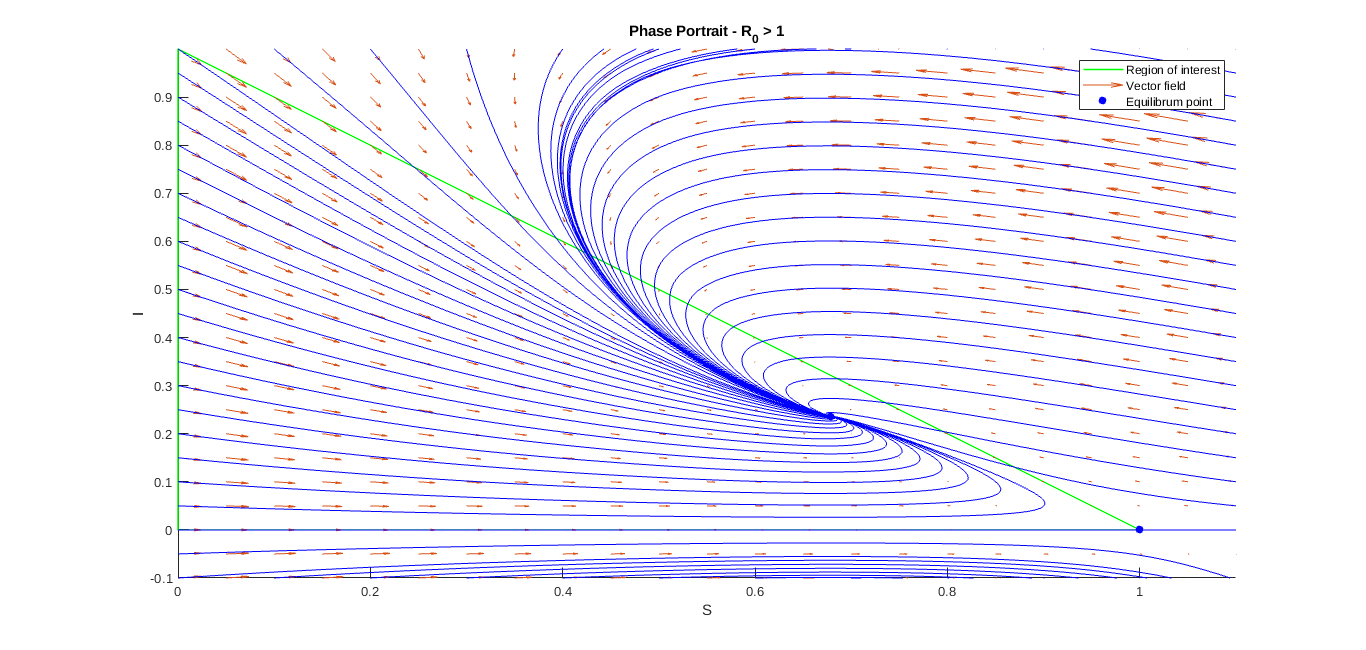
\includegraphics[scale=0.45]{Figure/pp_R0_major_1.png}
    \caption{Phase Plane of SIR model with $R_0 > 1$ and parameters $\beta = 0.4$, $\mu = 0.2$, $\gamma=\frac{1}{14}$}
    \label{fig:phase_plane_r0_major_1}
\end{figure}

\subsubsection{Stability analysis}
\begin{theorem}
Suppose that $R_0 > 1$. Then endemic equilibrium point is locally asymptotically stable in $\Omega_c \subset \Omega$, where $\Omega_c = \{\left(x_s,x_i\right) \in \mathbb{R}^2 : x_s > 0, x_i > 0, x_s + x_i < 1\}$.
\end{theorem}

\begin{proof}
Choosing as condidate Lyapunov function

\begin{equation}
    \label{eq:lyapunov_r0_major_1}
    V = P_1 \left[ x_s - x_s^*ln\left( \frac{x_s}{x_s^*} \right)\right] + P_2 \left[ x_i - x_i^*ln\left( \frac{x_i}{x_i^*} \right)\right]
\end{equation}

It obvious verify that

\begin{equation}
    x - c\ln\left(\frac{x}{c}\right) > 0 \;\;\; \forall x > 0, \; c > 0
\end{equation}

So, $V$ is positive for each point of $\Omega_c$.

\begin{equation}
    \label{eq:lyapunov_derivative_1_r0_major_1}
    \dot{V} = \frac{\partial V}{\partial x_s} \dot{x_s} + \frac{\partial V}{\partial x_i} \dot{x_i} = \left[ \frac{P_1}{x_s}(x_s - x_s^*) \right] \left[ \mu - \mu x_s - \beta x_i x_s \right] + \left[ \frac{P_2}{x_i}(x_i - x_i^*) \right] \left[ \beta x_i x_s - x_i (\gamma + \mu) \right]
\end{equation}

Given that

\begin{equation}
    \label{eq:x_s}
    x_s^* = \frac{\gamma + \mu}{\beta} \implies \gamma + \mu = \beta x_s^*
\end{equation}

Substituting \ref{eq:x_s} in \ref{eq:lyapunov_derivative_1_r0_major_1}, happens that

\begin{equation}
    \label{eq:lyapunov_derivative_2_r0_major_1}
    \dot{V} =  \frac{\left(x_s - x_s^*\right)}{x_s} \left[  P_1 \mu - P_1 \mu x_s - P_1\beta x_sx_i+P_2 \beta x_s \left( x_i - x_i^* \right) \right]
\end{equation}

Given that

\begin{equation}
    \label{eq:x_i}
    x_i^* = \frac{\mu}{\beta x_s^*} - \frac{\mu}{\beta} \implies \mu = \frac{\mu}{x_s^*} - \beta x_i^*
\end{equation}

Substituting \ref{eq:x_i} in \ref{eq:lyapunov_derivative_2_r0_major_1} happnes that

\begin{equation}
    \label{eq:lyapunov_derivative_3_r0_major_1}
    \dot{V} = \frac{P_1 \mu}{x_s^* x_s} \left( x_s - x_s^* \right)^2 + \beta \left( x_s - x_s^* \right)\left( x_i - x_i^* \right)\left( P_2 - P_1 \right)
\end{equation}

Choosing $P_1 = P_2 = P > 0$ happnes that

\begin{equation}
    \label{eq:lyapunov_derivative_4_r0_major_1}
    \dot{V} = \frac{P\mu}{x_s^* x_s} \left( x_s - x_s^* \right)^2
\end{equation}

Now
\begin{itemize}
    \item $ \dot{V} \leq 0 \;\;\;\;\; \forall \left( x_s, x_i \right) \in \Omega_c$
    \item $ \dot{V} = 0 \implies M = \{(x_s,x_i) \in\mathbb{R}^2: x_s = x_s^*\}$
    \item Largest invariant set in $M$ is $E = \{(x_s^*,x_i^*)\}$
\end{itemize}

So for the LaSalle invariant priciple the endemic equilibrium point is locally asymptotically stable in $\Omega_c$ \cite[p.128]{bib:khalil}.
\end{proof}

\begin{figure}[h!]
    \centering
    \label{fig:lyapunov_r0_major_1}
    \begin{subfigure}{\textwidth}
        \centering
        % include first image
        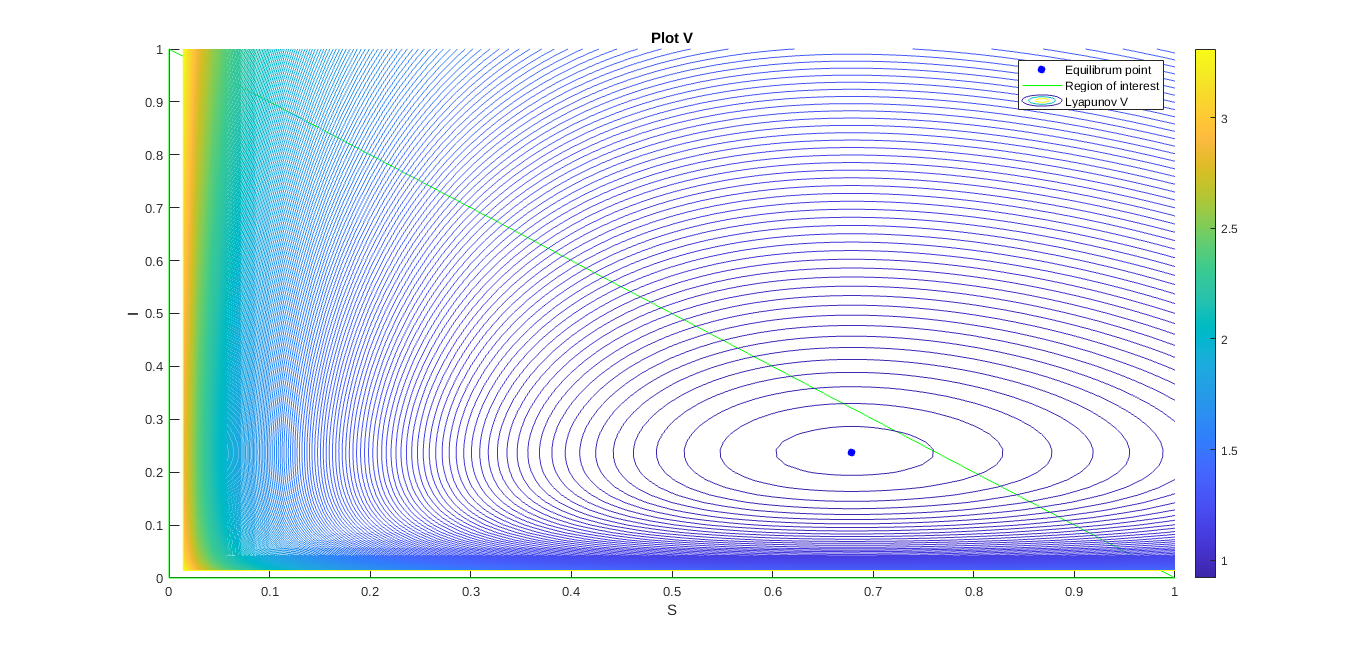
\includegraphics[width=\linewidth]{Figure/lyapunov_2d_R0_major_1.png}  
        \caption{V in 2D}
        \label{fig:lyapunov_r0_major_1_first}
    \end{subfigure}
    \begin{subfigure}{\textwidth}
        \centering
        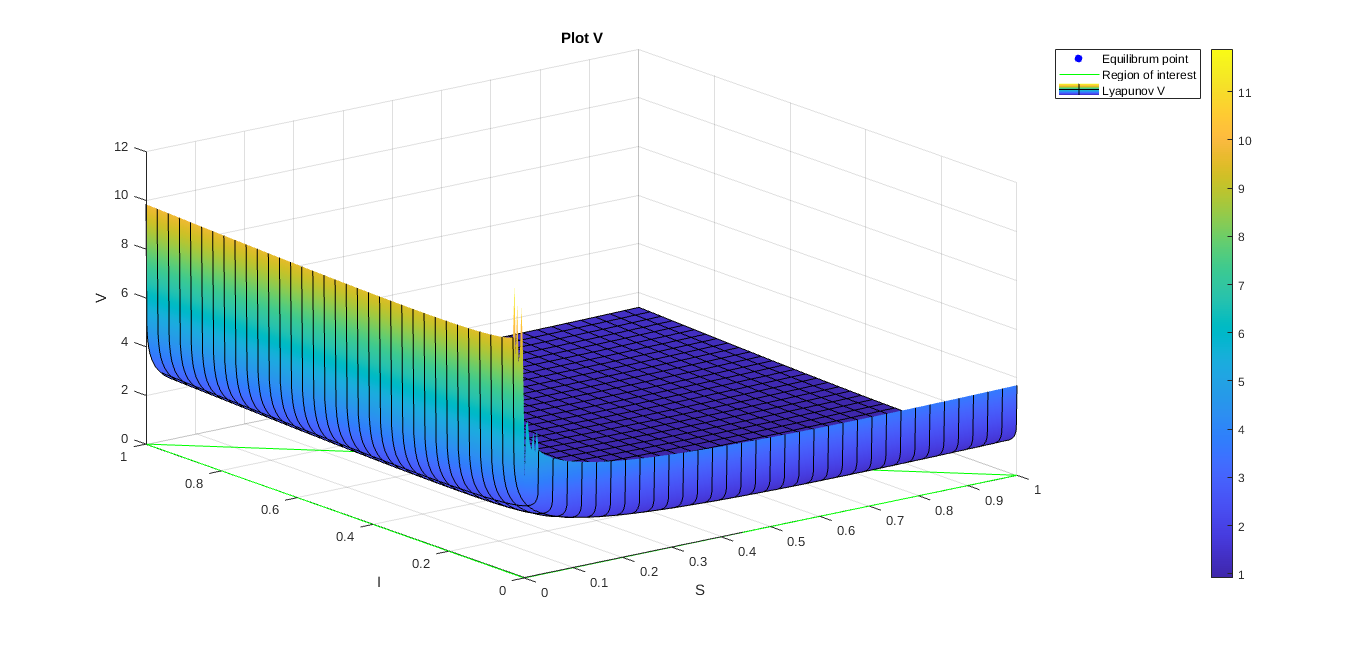
\includegraphics[width=\linewidth]{Figure/lyapunov_3d_R0_major_1.png}  
        \caption{V in 3D}
        \label{fig:lyapunov_r0_major_1_second}
    \end{subfigure}
    \caption{V with parameters $\beta = 0.4$, $\mu = 0.2$, $\gamma = \frac{1}{14}$, $P = 1$}
\end{figure}

\begin{figure}[h!]
    \centering
    \label{fig:lyapunov_derivative_r0_major_1}
    \begin{subfigure}{\textwidth}
        \centering
        % include first image
        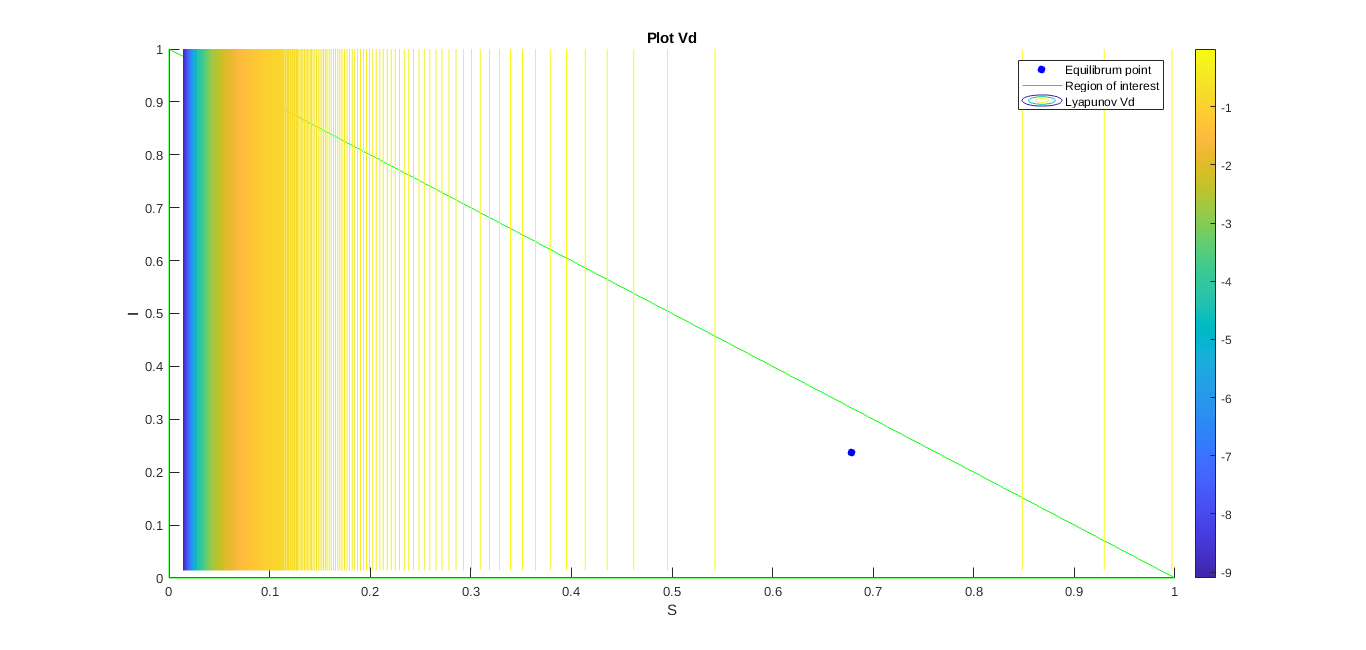
\includegraphics[width=\linewidth]{Figure/lyapunov_derivative_2d_R0_major_1.png}  
        \caption{$\dot{V}$ in 2D}
        \label{fig:lyapunov_derivative_r0_major_1_first}
    \end{subfigure}
    \begin{subfigure}{\textwidth}
        \centering
        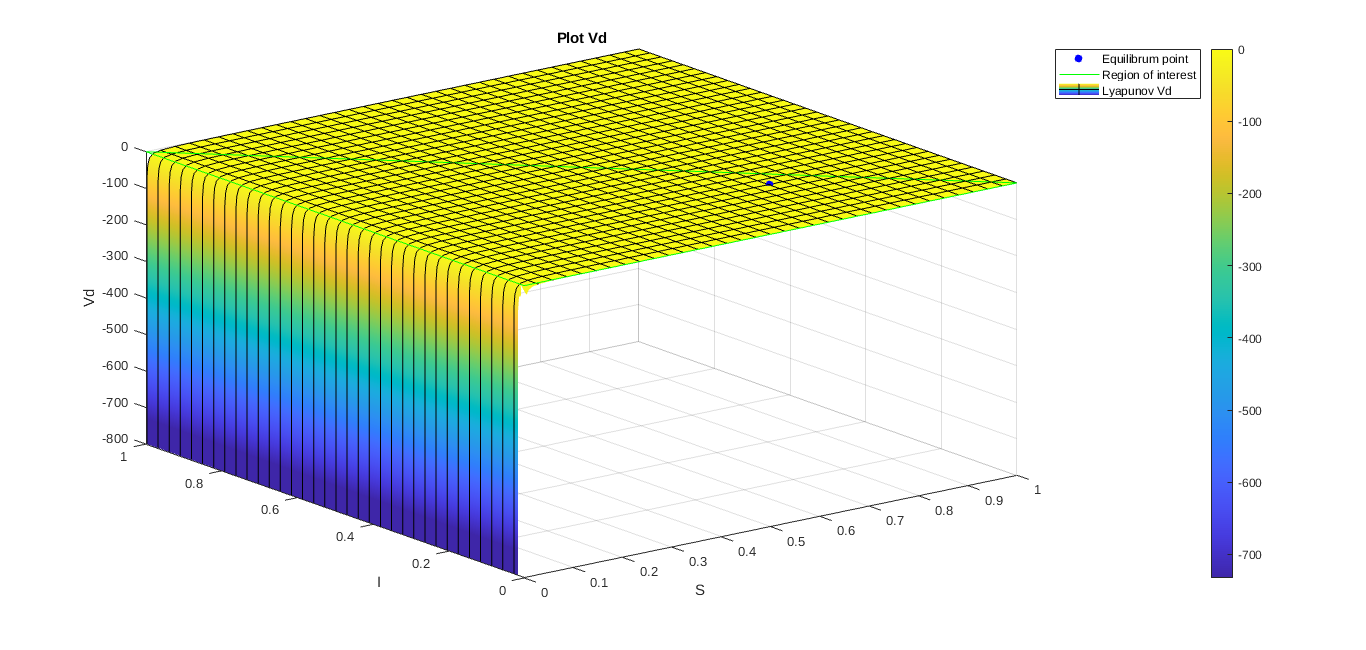
\includegraphics[width=\linewidth]{Figure/lyapunov_derivative_3d_R0_major_1.png}  
        \caption{$\dot{V}$ in 3D}
        \label{fig:lyapunov_derivative_r0_major_1_second}
    \end{subfigure}
    \caption{$\dot{V}$ with parameters $\beta = 0.4$, $\mu = 0.2$, $\gamma = \frac{1}{14}$, $P = 1$}
\end{figure}

\subsection{Bifurcation analsys}

First of all, it is important notice that, given \ref{eq:r0_definition} and given that $\beta$ and $\mu$ are intrinsic parameter that cannot be changed, and remembering that $R_0 = \frac{\beta}{\gamma + \mu}$, then

\begin{equation}
    R_0 = 1 \implies \gamma =  \beta - \mu
\end{equation}

As has been seen before, for $\gamma > \beta-\mu$ in $\Omega$ there is only one not endemic equilibrium point (node), while for $\gamma < \beta-\mu$ in $\Omega$ there are a not endemic equilibrium point (saddle point) and an endemic equilibrium point (stable focus or node). Actually, considering as domain not $\Omega$ but all $\mathbb{R}^2$ even to $R_0 < 1$ there is an endemic equilibrum point (saddle point).

Varing $\gamma < \beta-\mu$ happens that endemic equilibrium point (initially asymptotically stable) tend to became closer to not endemic equilibria (saddle point). At $\gamma = \beta-\mu$ there is a "crush" between them where stable manifold of endemic quilibria "changes" stability with unstable maniold of not endemic equilibrium point.
After this crush, for $\gamma > \beta-\mu$ endemic equilibrium point became a saddle point and go outside of $\Omega$, while not endemic equilibrium point became a stable node.

In Figure \ref{fig:bifurcation_s} and Figure \ref{fig:bifurcation_i} are rapresented variations of S e I:
\begin{itemize}
    \item dashed lines are associated with saddle point;
    \item continuous lines are associated with locally asymptotically stable point
\end{itemize}

\begin{figure}[h!]
    \label{fig:bifurcation}
    \begin{subfigure}{.5\textwidth}
        \centering
        % include first image
        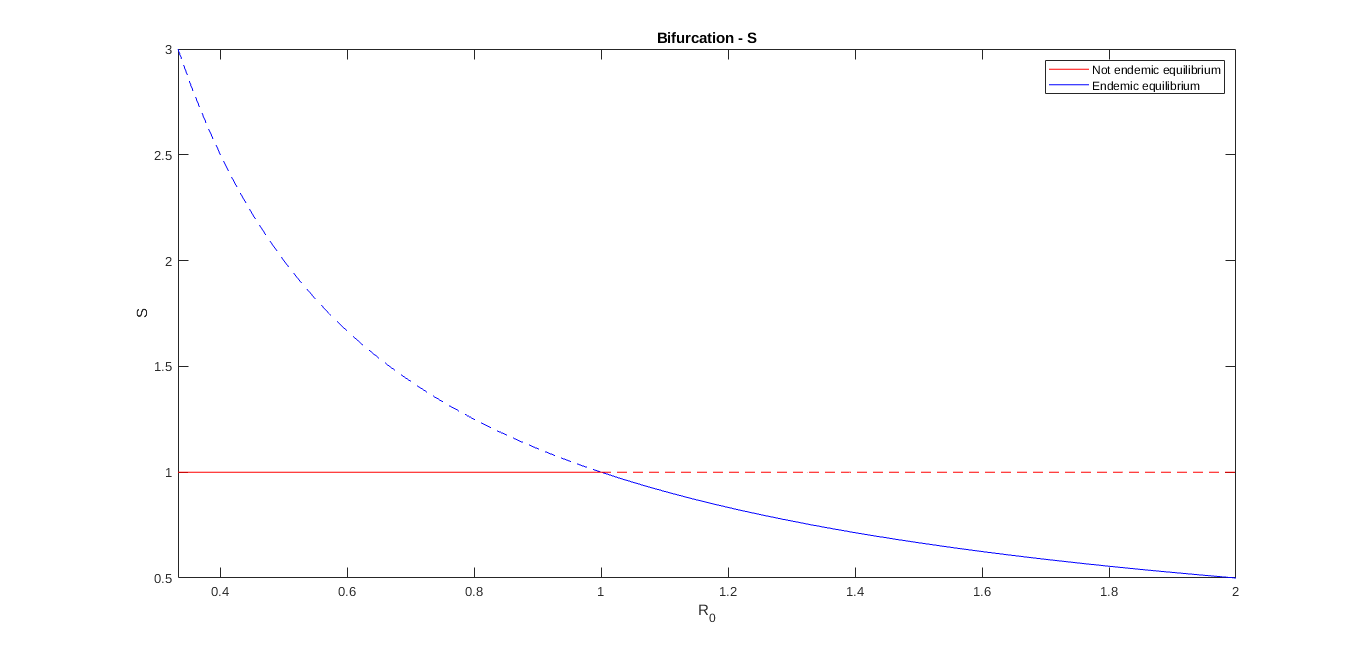
\includegraphics[width=\linewidth]{Figure/bifurcation_s.png}  
        \caption{Bifurcation of S}
        \label{fig:bifurcation_s}
    \end{subfigure}
    \begin{subfigure}{.5\textwidth}
        \centering
        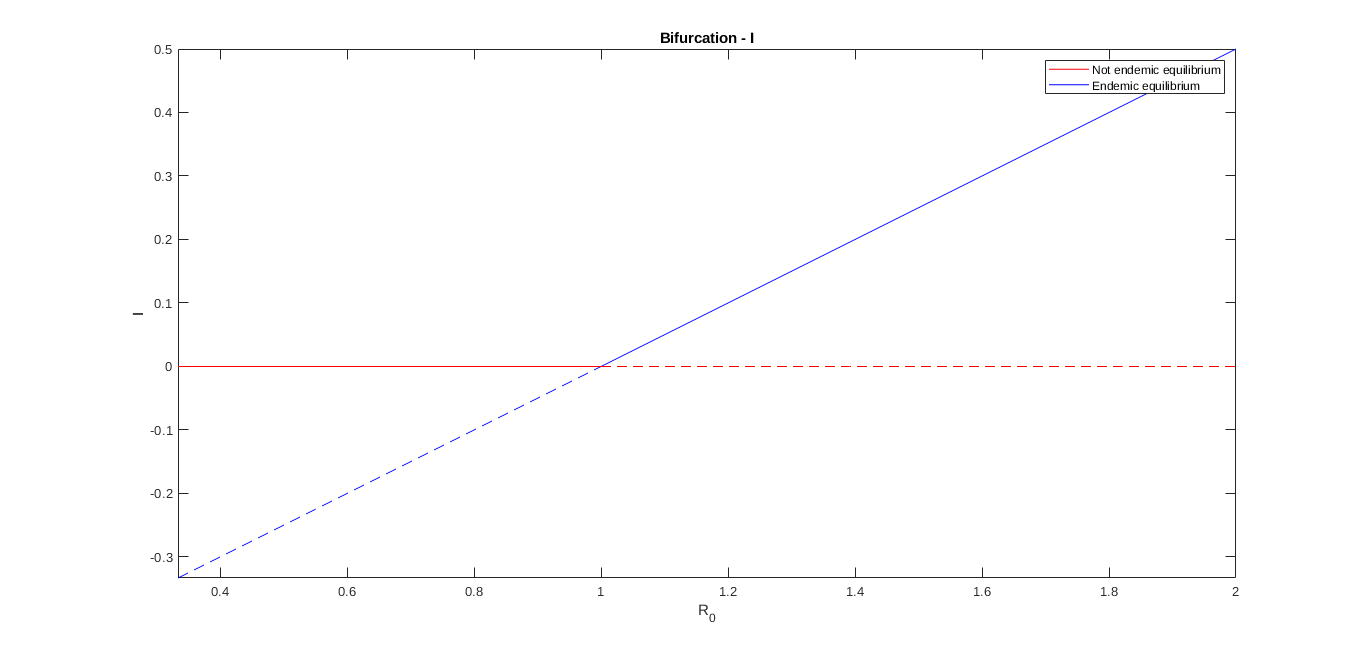
\includegraphics[width=\linewidth]{Figure/bifurcation_i.png}  
        \caption{Bifurcation of I}
        \label{fig:bifurcation_i}
    \end{subfigure}
    \caption{Bifurcation with parameters $\beta = 0.4$, $\mu = 0.2$,}
\end{figure}

\break
\begin{theorem}
$\gamma = \beta-\mu$ is a bifurcation point for System (\ref{eq:sir_model_3}). Moreover, in the neighborhood of $(x_s,x_i) = (1,0)$ system is topologically equivalent to normal form
\begin{equation}
    \dot{\xi} = \nu\xi + \xi^2 + O\left(\|(\xi,\nu)\|^3\right)
\end{equation}
\end{theorem}

\begin{proof}

First of all can be useful do a change of variables

\begin{equation}
    \label{eq:chage_of_variable_1}
    \begin{array}{ccc}
    x &=& x_s - 1 \\
    \dot{x} &=& \dot{x_s} \\
    y &=& x_i \\
    \dot{y} &=& \dot{x_i} \\
    \alpha &=& \beta - \gamma - \mu
    \end{array}
\end{equation}

Substituting Equation (\ref{eq:chage_of_variable_1}) in Equation (\ref{eq:sir_model_3}) it happens that:

\begin{equation}
    \label{eq:sir_model_4}
    \begin{array}{ccc}
        \dot{x} &=& -\mu x -\beta y - \beta xy \\
        \dot{y} &=& (\alpha+\beta) y +\beta xy
    \end{array}
\end{equation}

Where bifurcation point became $(x,y,\alpha) = (0,0,0)$.

Eigenvalues of System (\ref{eq:sir_model_4}) at bifurcation point are

\begin{equation}
    \begin{array}{ccc}
        \lambda_1 &=& -\mu \\
        \lambda_2 &=& \alpha
    \end{array}
\end{equation}

Eigenvector associated at eigenvalue $\lambda_1$ is
\begin{equation}
    \begin{pmatrix}
        0 & \beta \\ 0 & -\mu-\alpha-\beta
    \end{pmatrix}
    \begin{pmatrix}
        \alpha_1 \\ \alpha_2
    \end{pmatrix} =
    \begin{pmatrix}
        0 \\ 0
    \end{pmatrix}
    \implies
    \begin{pmatrix}
        1 \\ 0
    \end{pmatrix}
\end{equation}

Eigenvector associated at eigenvalue $\lambda_2$ is
\begin{equation}
    \begin{pmatrix}
        \alpha+\mu & \beta \\ 0 & 0
    \end{pmatrix}
    \begin{pmatrix}
        \alpha_1 \\ \alpha_2
    \end{pmatrix} =
    \begin{pmatrix}
        0 \\ 0
    \end{pmatrix}
    \implies
    \begin{pmatrix}
        1 \\ -\frac{\alpha+\mu}{\beta}
    \end{pmatrix}
\end{equation}

So locally at bifurcation point happens

\begin{equation}
    \label{eq:uv}
    \begin{pmatrix} x \\ y \end{pmatrix}
    = u
    \begin{pmatrix} 1 \\ 0 \end{pmatrix} + v
    \begin{pmatrix} 1 \\ -\frac{\alpha + \mu}{\beta}\end{pmatrix}
    \implies \begin{pmatrix} x \\ y \end{pmatrix}
    = \begin{pmatrix} u + v \\ -\frac{\alpha + \mu}{\beta} v \end{pmatrix}
\end{equation}

Consequentialy
\begin{equation}
    \label{eq:uv_dot}
    \begin{pmatrix} \dot{x} \\ \dot{y} \end{pmatrix}
    = \begin{pmatrix} \dot{u} + \dot{v} \\ -\frac{\alpha + \mu}{\beta} \dot{v} \end{pmatrix}
\end{equation}

Substituting Equation (\ref{eq:uv}) and Euqation (\ref{eq:uv_dot}) in Equation (\ref{eq:sir_model_4}), it happens

\begin{equation}
    \label{eq:sir_model_5}
    \begin{array}{ccc}
        \dot{u} &=& -\mu u + \left[ \beta(\alpha+\mu)-\beta \right]uv + \left[ \beta(\alpha + \mu) -\beta \right]v^2 \\
        \dot{v} &=& (\alpha + \beta u)v + \beta v^2
    \end{array}
\end{equation}

Given that eigeinvector associated with eigenvalue $\lambda_1$ is a stable manifold, while eigenvector associated with eigenvalue $\lambda_2$ is a center manifold, using Center Manifold Theorem \cite[pp. 303]{bib:khalil} locally at bifurcation point happens

\begin{equation}
    u = h(v,\alpha) = a+bv+c\alpha+dv^2+e\alpha^2+fv\alpha+O\left(\|(v,\alpha)\|^3\right)
\end{equation}

Moreover
\begin{equation}
    v = 0 \;\;\; \alpha = 0 \implies u = 0 \implies a = 0
\end{equation}

Then

\begin{equation}
    \label{eq:u_1}
    u = h(v,\alpha) = bv+c\alpha+dv^2+e\alpha^2+fv\alpha+O\left(\|(v,\alpha)\|^3\right)
\end{equation}

Now

\begin{equation}
    \label{eq:dotu_1}
    \dot{u} = \frac{\partial h}{\partial v}\dot{v} + \frac{\partial h}{\partial \alpha}\dot{\alpha} = \frac{\partial h}{\partial v}\dot{v} \;\;\;\; \text{in quanto} \;\;\;\; \dot{\alpha} = 0
\end{equation}

Remembering results of Equation (\ref{eq:u_1})

\begin{equation}
    \begin{array}{ccc}
        \frac{\partial h}{\partial v} &=& b + 2dv+f\alpha+O\left(\|(v,\alpha)\|^3\right) \\
        \dot{v} &=& \alpha v + \beta v^2 + \beta b v^2 + \beta bc \alpha v + O\left(\|(v,\alpha)\|^3\right)
    \end{array}
\end{equation}

Then 
\begin{equation}
    \label{eq:dotu_2}
    \dot{u} = (b+\beta bc)\alpha v + (\beta b + \beta b^2) v^2 + O\left(\|(v,\alpha)\|^3\right)
\end{equation}

Substituiting Equation (\ref{eq:u_1}) in Equation (\ref{eq:uv_dot}) it happens that
\begin{equation}
    \label{eq_dotu_3}
    \dot{u} = -(\mu b)v -(\mu c)\alpha +(-\mu d + \beta\mu b -\beta b+\beta\mu-\beta)v^2-(\mu e)\alpha^2+(-\mu f+\beta\mu c -\beta c)\alpha v+O\left(\|(v,\alpha)\|^3\right)
\end{equation}

Comparing Equation (\ref{eq:dotu_2}) with Equation (\ref{eq_dotu_3}) and, solving the system, it happens that

\begin{equation}
    \label{eq:coefficients}
    \begin{array}{ccc}
        b &=& 0 \\
        c &=& 0 \\
        d &=& \beta-\frac{\beta}{\mu} \\
        e &=& 0 \\
        f &=& 0
    \end{array}
\end{equation}

Substituiting Equation (\ref{eq:coefficients}) in Equation (\ref{eq:u_1}) it happens
\begin{equation}
    u = \left(\beta - \frac{\beta}{\mu}\right) v^2 + O\left(\|(v,\alpha)\|^3\right)
\end{equation}

So equation associted to critic eigenvector
\begin{equation}
    \dot{v} = \alpha v + \beta v^2 + O\left(\|(v,\alpha)\|^3\right)
\end{equation}

Defining $\nu = \alpha$ and $v = \frac{\xi}{\beta}$ siit happens

\begin{equation}
    \dot{\xi} = \nu\xi + \xi^2 + O\left(\|(\xi,\nu)\|^3\right)
\end{equation}
\end{proof}

\subsection{Simulazioni}
Di seguito verranno riportate due simulazioni del modello SIR.

In Figure \ref{fig:sir_model_evolution_r0_minor_1} is rapresented the evolution of SIR model in case of $R_0 < 1$. It should be noted that Infected tends towards zero because sum of recovery rate and death rate are major then infection rate, so number of people that are infected are less then number of people that are healed by national healthcare system. Removed tends towards zero because birth rate is equal to death rate, so for each people that dies, onther one born in Susceptible.

\begin{figure}[h!]
    \centering
    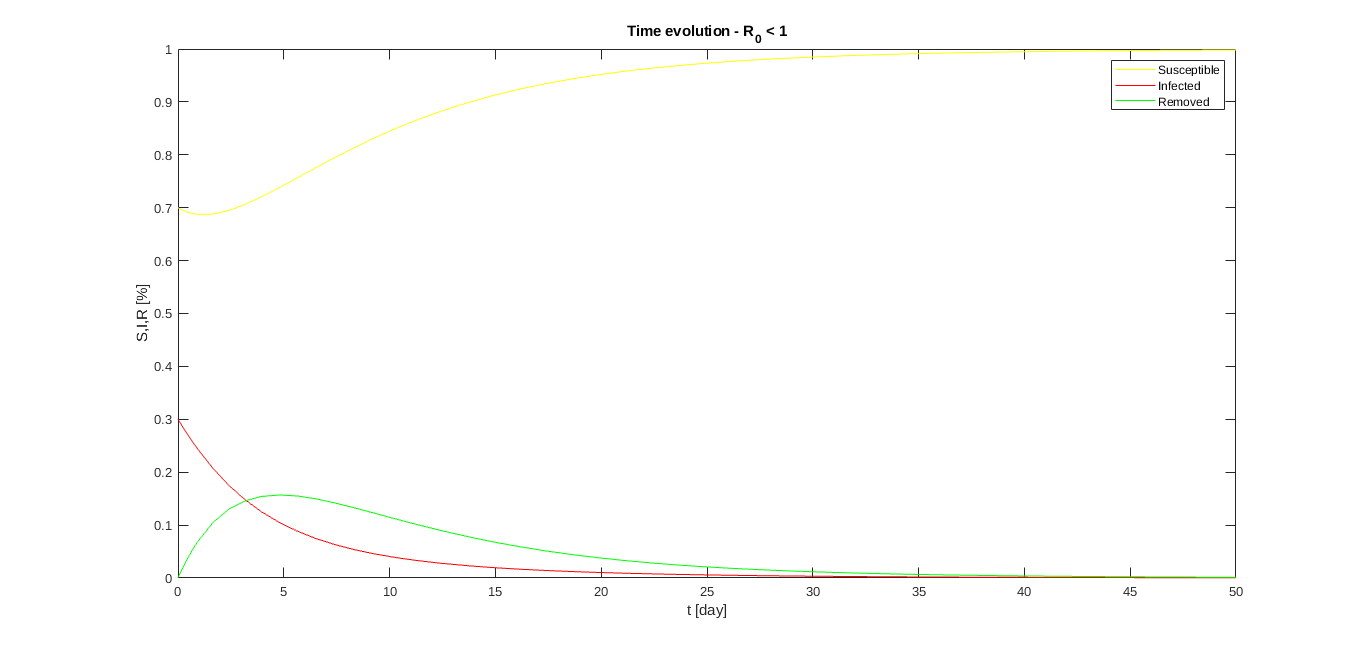
\includegraphics[width=\linewidth]{Figure/SIR_evolution_r0_minor_1.png}
    \caption{Evolution of SIR model with parameters $\beta = 0.4$, $\mu = 0.2$, $\gamma = 0.3$}
    \label{fig:sir_model_evolution_r0_minor_1}
\end{figure}

In Figure \ref{fig:sir_model_evolution_r0_major_1} is rapresented the evolution of SIR model in case of $R_0 > 1$. It should be noted that Infected tends towards a value different from zero, this because health care system cannot heal in time all infected, so national healthcare system saturates and a constant part of infected die for other causes.

\begin{figure}[h!]
    \centering
    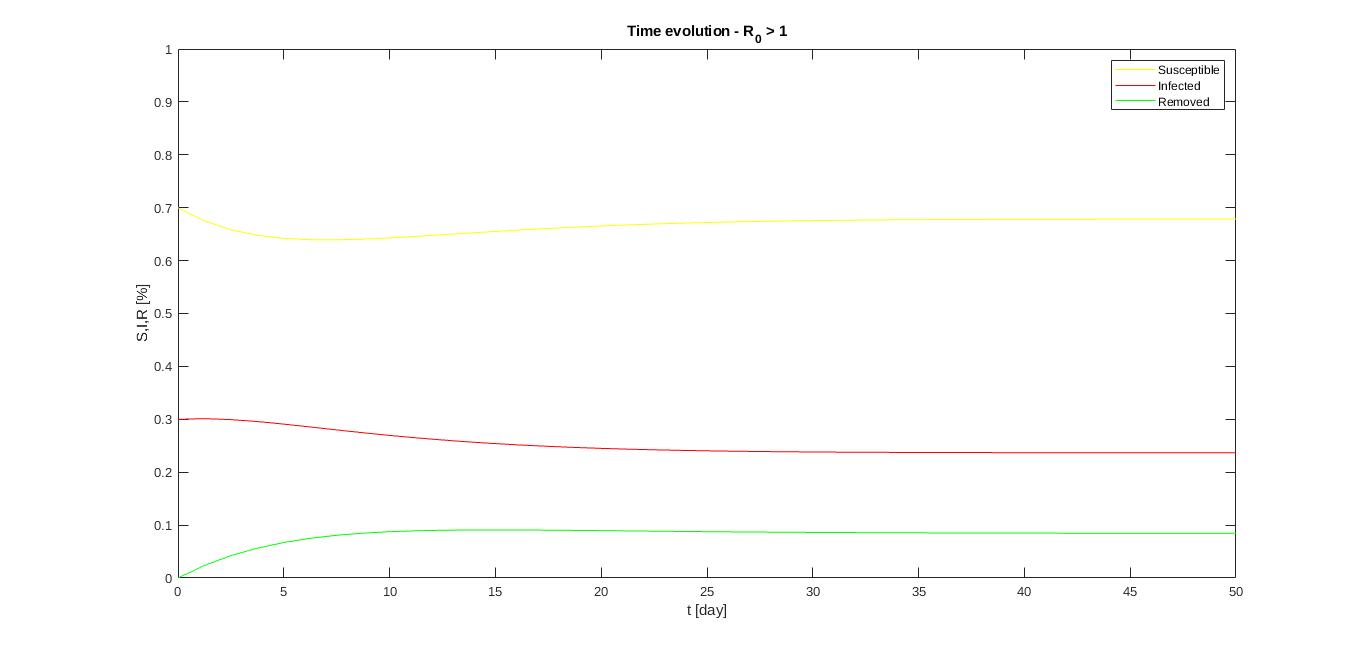
\includegraphics[width=\linewidth]{Figure/SIR_evolution_r0_major_1.png}
    \caption{Evolution of SIR model with parameters $\beta = 0.4$, $\mu = 0.2$, $\gamma = \frac{1}{14}$}
    \label{fig:sir_model_evolution_r0_major_1}
\end{figure}